\section{Implementation}

\subsection{Instruction set}

We chose 22 to be our instruction bit width, as it was sufficient for our requirements. We distinguish between three types of instructions:

\begin{center}
	\begin{tabular}{ | c | c | c | c | }
		\multicolumn{4}{c}{\textbf{R-Type}} \\
		\hline
		\textbf{Operation Code} & \textbf{Destination Register} & \textbf{Source Register} & \textbf{Function Code} \\
		\hline
		6 bit & 5 bit & 5 bit & 6 bit \\
		\hline
	\end{tabular} 
\end{center}

\begin{center}
	\begin{tabular}{ | c | c | c | }
		\multicolumn{3}{c}{\textbf{I-Type}} \\
		\hline
		\textbf{Operation Code} & \textbf{Destination Register} & \textbf{Immediate} \\
		\hline
		6 bit & 5 bit & 11 bit \\
		\hline
	\end{tabular} 
\end{center}

\begin{center}
	\begin{tabular}{ | c | c | }
		\multicolumn{2}{c}{\textbf{J-Type}} \\
		\hline
		\textbf{Operation Code} & \textbf{Jump Address} \\
		\hline
		6 bit & 16 bit \\
		\hline
	\end{tabular} 
\end{center}

Our instruction set consists of the following instructions: 

\begin{center}
	\begin{tabular}{ | c | c | c | c |}
		\hline
		Operation & Op-Code & Type & Func-Code \\
		\hline
		ADC\_IN	& 0b000001	& R	& 0b000000	\\
		MUL	& 0b000010	& R	& samt	\\
		SIN	& 0b000011	& R	& 0b000000	\\
		MOV	& 0b000100	& R	& 0b000000	\\
		ADD	& 0b000101	& R	& 0b000000	\\
		SUB	& 0b000110	& R	& 0b000000	\\
		INC	& 0b000111	& R	& 0b000000	\\
		CP	& 0b001000	& R	& 0b000000	\\
		DAC\_OUT	& 0b001001	& R	& 0b000000	\\
		AND	& 0b001010	& R	& 0b000000	\\
		OR	& 0b001011	& R	& 0b000000	\\
		XOR	& 0b001100	& R	& 0b000000	\\
		SLL	& 0b001101	& R	& 0b000000	\\
		SRL	& 0b001110	& R	& 0b000000	\\
		SRA	& 0b001111	& R	& 0b000000	\\
		WAIT	& 0b111111	& R	& 0b000000	\\
		MOVI	& 0b010100	& I	& N/A	\\
		ADDI	& 0b010101	& I	& N/A	\\
		ANDI	& 0b011010	& I	& N/A	\\
		ORI	& 0b011011	& I	& N/A	\\
		XORI	& 0b011100	& I	& N/A	\\
		SLLI	& 0b011101	& I	& N/A	\\
		SRLI	& 0b011110	& I	& N/A	\\
		SRAI	& 0b011111	& I	& N/A	\\
		JMP	& 0b100000	& J	& N/A	\\
		JC	& 0b100001	& J	& N/A	\\
		JNC	& 0b100010	& J	& N/A	\\
		JZ	& 0b100011	& J	& N/A	\\
		JNZ	& 0b100100	& J	& N/A	\\
		JN	& 0b100101	& J	& N/A	\\
		JNN	& 0b100110	& J	& N/A	\\
		\hline
	\end{tabular} 
\end{center}

As this instruction set is very similar to many common assembly instrucion sets, it is very intuitive for a programmer to use it. 

To translate our pseudo assembly code into binary, we wrote a translater script in python.

\subsection{Registers}

We settled for an amount of 25 registers. This is more than enough to fit our needs:

\begin{center}
	\begin{tabular}{ | c | c | c |}
		\hline
		Register	& Reg-Code	& Symbol	\\
		\hline
		Reg0	& 0b00001	& r0	\\
		Reg1	& 0b00010	& r1	\\
		Reg2	& 0b00011	& r2	\\
		Reg3	& 0b00100	& r3	\\
		Reg4	& 0b00101	& r4	\\
		Reg5	& 0b00110	& r5	\\
		Reg6	& 0b00111	& r6	\\
		Reg7	& 0b01000	& r7	\\
		Reg8	& 0b01001	& r8	\\
		Reg9	& 0b01010	& r9	\\
		Reg10	& 0b01011	& r10	\\
		Reg11	& 0b01100	& r11	\\
		Reg12	& 0b01101	& r12	\\
		Reg13	& 0b01110	& r13	\\
		Reg14	& 0b01111	& r14	\\
		Reg15	& 0b10000	& r15	\\
		Reg16	& 0b10001	& r16	\\
		Reg17	& 0b10010	& r17	\\
		Reg18	& 0b10011	& r18	\\
		Reg19	& 0b10100	& r19	\\
		Reg20	& 0b10101	& r20	\\
		RegY\_L	& 0b10110	& y\_L	\\
		RegY\_H	& 0b10111	& y\_H	\\
		RegZ\_L	& 0b11000	& z\_L	\\
		RegZ\_H	& 0b11001	& z\_H	\\
		\hline
	\end{tabular} 
\end{center}

The registers \textit{RegY\_L}, \textit{RegY\_H}, \textit{RegZ\_L}, \textit{RegZ\_H}
were planned to hold a multiplication result, but are currently not used in any special way.

\subsection{Status register} 

In the status register, we store a zero flag, negative flag and overflow flag of the last operation performed by the \textit{exec\_stage}. 

\subsection{Structure}

We structured our microcontroller in the form of four stages a operation has to go through until it is considered executed: Fetch stage, Decode stage, Execution stage and Writeback stage.
We used this semantic divide of the process to structure our VHDL entities in the same way.

A screenshot of the RTL view can be found in figure \ref{fig:block}

\subsubsection{Fetch stage}

\begin{center}
	\begin{tabular}{ | l | c | l | }
		\hline
		\textbf{Portname} & \textbf{Direction} & \textbf{Description} \\
		\hline
		clk & in & Clock signal \\
		reset & in  & Reset signal \\
		start & in  & Start signal \\
		done & out  & Done signal \\
		jmp & in  & Flag that decides if the jmp\_addr should be used as next PC or not \\
		jmp\_addr & in  & Jump address \\
		instr & out  & Instruction in binary to be decoded by the decode stage \\
		\hline
	\end{tabular} 
\end{center}


The fetch stage holds the instruction memory. In our case, the instruction memory is a constant array of std\_logic\_vectors with a width of 22 bit. The program counter (PC) is used as index to access the array. The std\_logic input port \textit{jmp} decides if the new PC should be the old PC + 1 or the \textit{jmp\_addr}. 

\subsubsection{Decode stage}

\begin{center}
	\begin{tabular}{ | l | c | l | }
		\hline
		\textbf{Portname} & \textbf{Direction} & \textbf{Description} \\
		\hline
		clk & in & Clock signal \\
		reset & in  & Reset signal \\
		start & in  & Start signal \\
		done & out  & Done signal \\
		instr & in  & Instruction in binary that will be decoded in this stage \\
		wr & in  & Flag that determines if there should be a write operation on the register file \\
		wraddr & in  & The register address where data will be written to \\
		wrdata & in  & The data that will be written in the register file  \\
		exec\_op & out  & The decoded instruction structure to be passed to the exec stage \\
		\hline
	\end{tabular} 
\end{center}

The decode stage holds the register file (regfile). It writes to the regfile and reads from the regfile according to it's inputs. It fills the exec\_op data structure that determines which operation will be executed by the execution stage.

\subsubsection{Execution stage}

\begin{center}
	\begin{tabular}{ | l | c | l | }
		\hline
		\textbf{Portname} & \textbf{Direction} & \textbf{Description} \\
		\hline
		clk & in & Clock signal \\
		reset & in  & Reset signal \\
		start & in  & Start signal \\
		done & out  & Done signal \\
		op & in  & Data structure that holds the decoded instruction \\
		result & out  & Multiplexed result of the executed operation \\
		writeback & out  & Flag that determines if the result should be written back into the regfile \\
		rd & out  & Destination register \\
		jmp & out  & Flag that determines if a jump should be performed or not \\
		adc\_rddata & in  & Data read from the ADC \\
		dac\_wrdata & out  & Data to be written to the DAC \\
		dac\_valid & out  & Valid flag for the DAC \\
		\hline
	\end{tabular} 
\end{center}

As the name suggests, the execution stage executes the decoded operation. It holds the arithmetical logical unit (ALU), the sine cordic component from task 1, a wait unit for artificial delay and our multiplication unit. It also holds the status register (zero flag, negative flag, overflow flag) to determine if a conditional jump should be performed or not.

For the ADC and DAC operations in our instruction set, it writes data to the ports \textit{dac\_valid} and \textit{dac\_wrdata} and reads from the port \textit{adc\_rddata}.

\subsubsection{Writeback stage}

\begin{center}
	\begin{tabular}{ | l | c | l | }
		\hline
		\textbf{Portname} & \textbf{Direction} & \textbf{Description} \\
		\hline
		clk & in & Clock signal \\
		reset & in  & Reset signal \\
		start & in  & Start signal \\
		done & out  & Done signal \\
		writeback & in  & Flag that determines if the result should be written back into the regfile \\
		rd & out  & Destination register \\
		data & out  & Data to be written into the regfile \\
		wr & out  & Flag that determines if the result should be written back into the regfile \\
		wraddr & out  & The register address where data will be written to \\
		wrdata & in  & The data that will be written in the register file \\
		jmp\_in & out  & Flag that determines if a jump should be performed or not  \\
		jmp\_out & out  & Flag that determines if a jump should be performed or not \\
		jmp\_addr & out  & Jump address \\
		\hline
	\end{tabular} 
\end{center}

The writeback stage is merely a relic of our initial pipeline design. It just shifts data from the exec stage to the fetch and decode stage. We kept it for possible future expansion of the processor (with a RAM for example).

\subsubsection{Frequency Modulation Micro Controller (FMUC)}

\begin{center}
	\begin{tabular}{ | l | c | l | }
		\hline
		\textbf{Portname} & \textbf{Direction} & \textbf{Description} \\
		\hline
		clk & in & Clock signal \\
		reset & in  & Reset signal \\
		adc\_rddata & in  & Data read from the ADC \\
		dac\_wrdata & out  & Data to be written to the DAC \\
		dac\_valid & out  & Valid flag for the DAC \\
		\hline
	\end{tabular} 
\end{center}

The FMUC is our top component in which we wire all the stages together. 

\subsection{Xilinx Project Properties}

\subsubsection{Device Utilization}

\begin{figure}[!htb]
	%\centering % centering figure 
	\scalebox{1.00} % rescale the figure by a factor of 0.8 
	{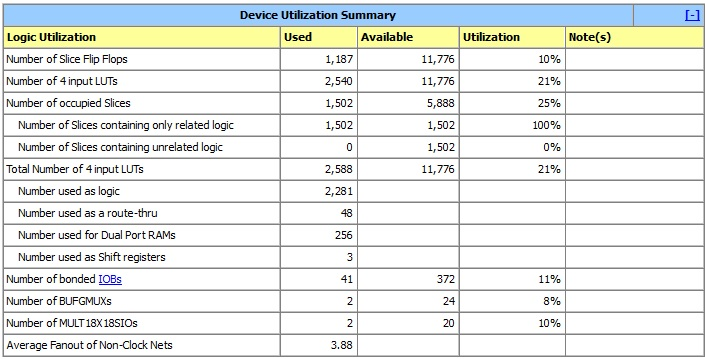
\includegraphics[height=6cm]{images/util.jpg}} % importing figure
	\caption{Device utilization report of Xilinx ISE} 
	\label{fig:util} % labeling to refer it inside the text
\end{figure} 

\subsubsection{Timing Summary}

\begin{lstlisting}
Minimum period: 16.002ns (Maximum Frequency: 62.493MHz)
Minimum input arrival time before clock: 1.521ns
Maximum output required time after clock: 12.918ns
Maximum combinational path delay: No path found
\end{lstlisting}

The phenomenon of the seemingly inexistent combinational path has already occured in task 2 and
is reoccuring in this project.

\newpage

\subsection{Program Code}
\begin{adjustwidth}{-4.3cm}{}
	\begin{lstlisting}
	MOVI	r1,0x00		# r1 = current sine angle
	MOVI	r2,0x00		# r2 = last ADC value
	MOVI 	r4,0x04		# r4 = angle step size for a baudrate of 44kHz
	SLLI	r4,0d08		# 
	ORI 	r4,0x92		# 
	MOVI	r5,0x00		# r5 = last sine angle
	MOVI	r6,0x64		# r6 = Pi
	SLLI	r6,0d08		# 
	ORI 	r6,0x84		# 
	MOVI	r7,0d530	# r7 = cycles to wait for carrier frequency (1khz)
	SLLI	r7,0d1		# 
	MOVI	r8,0x40		# r8 holds 2.0 fixpoint
	SLLI	r8,0d8		# 
	ADC_IN  r9		# r9 holds ADC output (between -1 and 1). LABEL: loop_start
	MOV 	r10,r9		# 
	ADD 	r10,r8		# add 2.0 fixpoint to ADC value to bring between 1 and 3
	MOV     r11,r10		# 
	SRLI    r11,0x01	# shift one right to divide by 2
	MOV     r12,r11		# 
	MUL     r12,r7,0x0D	# multply shifted DAC value with base wait cycle amount
	SIN 	r5		# calculate sine from current angle
	DAC_OUT	r5		# write last sine result to DAC
	ADD 	r1,r4		# increment angle
	CP  	r6,r1		# compare current angle with Pi
	JNN 	0d27		# jump to LABEL if_smaller_pi
	SUB 	r1,r6		# subtract Pi from current angle
	SUB 	r1,r6		# subtract Pi from current angle
	MOV 	r5,r1		# move current angle into r1. LABEL: if_smaller_pi
	WAIT	r12		# wait for the amount of cycles stored in r12
	JMP 	0d13		# jump to LABEL loop_start
	\end{lstlisting}
\end{adjustwidth}

\begin{landscape}
	\begin{figure}[H] 
		%\centering % centering figure 
		\scalebox{2.6} % rescale the figure by a factor of 0.8 
		{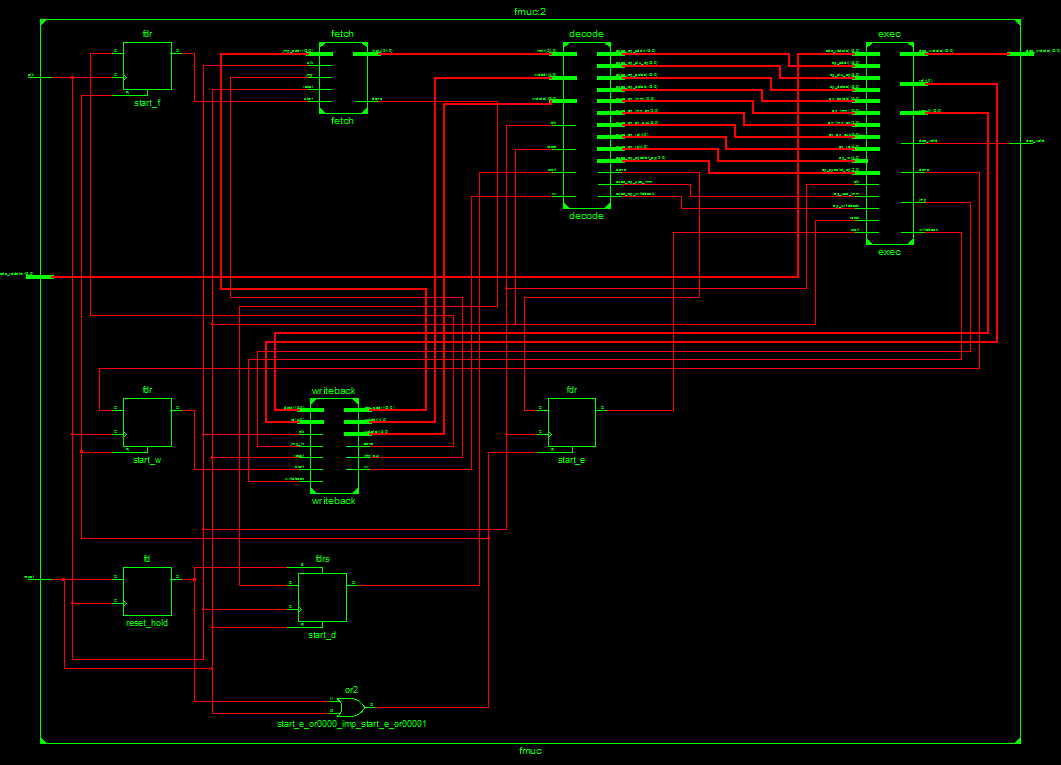
\includegraphics[height=6cm]{images/block_diagramm_rtl.jpg}} % importing figure
		\caption{RTL view of the FMUC} 
		\label{fig:block} % labeling to refer it inside the text
	\end{figure} 
\end{landscape}




 
